\chapter{Aprendizado de Máquina}
\section{Definição}
O termo Aprendizado de Máquina do inglês \textit{Machine Learning}, é considerado uma disciplina dentro da área da Inteligência Artificial, com foco na construção de softwares computacionais, dotados da capacidade de aprender autonomamente \cite{Hosch}. Essa disciplina trabalha com o estudo e a construção de algoritmos, capazes de aprender com seus “erros” no reconhecimento de dados e realizarem previsões sobre novos dados. Esses algoritmos de indução são considerados um grande passo na descoberta do conhecimento \cite{Kohavi}.

Apesar da complexidade em AM, essa disciplina pode ser contextualizada de maneira mais geral como o campo de estudo, que dá ao computador a habilidade de aprender sem ser explicitamente programado \cite{Arthur}, porém uma visão mais orientada para a área da engenharia, que segundo \citeonline{Tom}, é dito que um programa de computador aprende com a experiência “E” em relação a alguma tarefa “T” e alguma medida de desempenho “P”, se seu desempenho em “T” e medido por “P” melhora com a experiência “E” \cite{Tom}.

\section{Aplicações em Aprendizado de Máquina}
O AM serve de auxílio para diversos contextos de naturezas diferentes, sendo assim consegue auxiliar com o uso de dados históricos para escolher a melhor decisão de um negócio, como por exemplo uma possível aplicação de um modelo de AM é predizer qual a probabilidade de um cliente comprar um determinado produto com base no seu histórico de compras passadas \cite{Amazon}. Este trabalho de conclusão de curso, tem por objetivo geral trabalhar com a aplicação de um modelo de AM na área da saúde, sendo que já existem estudos semelhantes que já evidenciaram os resultados da utilização desses modelos neste contexto.

Na saúde AM, é uma tendência crescente na indústria médica, graças ao advento de dispositivos eletrônicos como sensores, que podem acessar aos dados de pacientes em tempo real. A tecnologia também pode ajudar médicos a analisar os dados para identificar tendências ou alertas, consequentemente levando ao aperfeiçoamento de diagnósticos e tratamentos \cite{Sas}.

\section{Funcionamento de um algoritmo de AM}
Cada algoritmo tem suas peculiaridades quanto ao seu funcionamento, entretanto esses algoritmos em seu estado mais básico trabalham com a entrada de dados num sistema, que processa os mesmos utilizando um modelo de predição geralmente já postulado, no qual derivam um resultado que referente a uma predição que o modelo fez sobre os dados de entrada. Esses algoritmos possuem alguns métodos e técnicas para validar seu funcionamento, por exemplo declarando uma dada porcentagem para avaliar o grau da acurácia de seu resultado, permitindo assim verificar se a predição gerada pelo algoritmo se aproxima do resultado esperado no contexto real. Sendo esse e outras situações melhor contextualizado neste capítulo.

Considerando ainda que o AM, com seu foco na predição no desenvolvimento de algoritmos capazes de aprender com seus erros, essa disciplina é muito atrelada a otimização matemática, além de que uma de suas principais características, é a utilização de métodos estatísticos para validar o seu funcionamento, sendo que todos esses aspectos matemáticos estão ligados à complexidade computacional o que em linhas gerais é a representação de um algoritmo de AM.

\section{Tipos de Aprendizado}
Os algoritmos são classificados quanto ao seu tipo de aprendizado, existindo três categorias que se distinguem de acordo com a natureza do comportamento no tratamento dos dados, estas categorias são aprendizado supervisionado, não supervisionado e por reforço \cite{geron2017hands}.
 
\subsection{Aprendizado Supervisionado}
O objetivo principal do aprendizado supervisionado é ensinar um modelos através de uma base de treino etiquetada, que nos permite fazer predições de dados futuros. O termos supervisionado se refere a um grupo de dados onde a "resposta", sinal ou valor esperado já é conhecido, este valor é conhecido como etiqueta. As tarefas do aprendizado supervisionado podem ser divididas em classificação e regressão, onde a classificação tem as etiquetas esperadas com um valor fixo, por exemplo uma avaliação binária, e a regressão é referente a um sinal com valor contínuo, como uma regressão polinomial \cite{geron2017hands}, ou segundo \cite{kirk2014thoughtful} é ajustar o conjunto de dados á uma função qualquer.

Exemplos de algoritmos existentes \cite{kirk2014thoughtful}:
\begin{itemize}
    \item \textit{\textbf{KNN}, K-Nearest Neighbor}: (K vizinhos mais próximos) Determina o rótulo de classificação de um dado baseando nos valores das amostras vizinhas mais próximos \cite{kirk2014thoughtful};
    \item \textit{Decision Trees}: é uma forma de organizar regras referentes a dados com estruturas hierárquicas e sequências, que particionam estes dados recursivamente \cite{murthy1998automatic};
    \item \textit{Support Vector Machines (SVMs)}: separado em linear e não linear, consiste na separação de dados de um conjunto maior em classes de conjuntos mais restritos \cite{lorena2007introduccao};
\end{itemize}

\subsection{Aprendizado não-supervisionado}
Ao contrário do aprendizado supervisionado, os dados não estão etiquetados ou até mesmo possuem uma estrutura desconhecida. Utilizando as técnicas do aprendizado não supervisionado é possível explorar a estrutura para extrair informações necessárias dos dados sem a orientação de uma variável de resultado conhecida ou uma função de recompensa \cite{geron2017hands} .

Exemplos de algoritmos existentes \cite{kirk2014thoughtful}:
\begin{itemize}
    \item \textit{Clustering}: É utilizado para agrupar padrões, ou melhor, no treinamento é introduzido um conjunto de dados e o algoritmo procura relações entre eles agrupandos tais dados em grupos por grau de semelhança, na predição, com um novo dado inserido o algoritmo busca padrões existentes nele e cataloga-o no respectivo grupo \cite{kirk2014thoughtful}.   
    \item \textit{Collaborative Filtering}: É utilizado no desenvolvimento de sistemas de recomendação, basicamente utiliza informações cruzadas dos usuários para predizer gostos em comum, por exemplo se você compra bastante cerveja em um site de compras, o sistema recomendará cerveja para você, caso um grupo significante de usuários compre cerveja e carvão, o sistema recomendará conjuntamente o carvão. \cite{kirk2014thoughtful}.  
\end{itemize}

\subsection{Aprendizado por reforço} 
Utiliza um sistema de recompensas para reforçar a continuidade de um comportamento esperado, como por exemplo um jogo onde o personagem é beneficiado com uma recompensa sempre que atinge um golpe no adversário, quanto mais forte for o golpe maior a recompensa, deste modo o modelo memoriza quais os comandos geraram as maiores recompensas \cite{kirk2014thoughtful}.

\section{\textit{Feature}}
Uma \textit{feature} é uma característica ou variável do problema, que pode ser processada pelo modelo e gerar um resultado condicente com a realidade, deve ser mensurável e independente, sendo que uma \textit{feature} é a base para o funcionamento dos algoritmos de classificação, regressão e reconhecimento de padrões, normalmente é um numero, mas pode ser uma palavra, grafo, vetor etc \cite{chandrashekar2014survey}.

A ainda um conceito importante sobre AMs, a \textbf{Redução de dimensionalidade}, muito utilizada em estatística e AM, refere-se ao processo de diminuição do número de variáveis aleatórias, selecionando um subconjunto com variáveis relevantes. Serve dentre outras funcionalidades, para transformar o processo de aprendizado mais eficiente \cite{borges2006reduccao}, isto ocorre devido a modelos com centenas de variáveis podem acarretar em um maior tempo de computação e um baixo desempenho da previsão \cite{chandrashekar2014survey}.

\section{Desafios do Aprendizado de Máquinas}
Em um projeto de AM, existem diversos aspectos que podem levar a um péssimo resultado ou problemas na execução do mesmo, em resumo, a tarefa principal do AM é a seleção de um algoritmo, ou modelo, e treiná-lo utilizando algum tipo de dado, logo ao analisar os problemas de um provenientes de um péssimo resultado, pode se o encontrar principalmente duas origens para o problema a escolha de um "algoritmo ruim" ou  "dados ruins".\cite{geron2017hands}.

O conceito de "dados ruins", não deve ser considerado ao pé da letra, sendo um pouco mais complexo, e envolve principalmente a coleta destes e tratamento associado. Para exemplificar,  pode-se listar alguns exemplos retirados do livro \cite{geron2017hands}:

\begin{itemize}
    \item \textbf{Quantidade insuficiente de dados de treino}: Para um funcionamento pleno de um sistema de AMs é necessário uma grande quantidade de dados, alguns problemas necessitam de uma alta quantidade de dados para funcionar corretamente, como no reconhecimento de imagens.
    \item \textbf{Dados não representativos}: Com o intuito de alcançar a boa generalização, é crucial que os dados de treino sejam representativos.
    \item \textbf{Dados de baixa qualidade}: É evidente que caso os dados de treinos tenham muitos erros e ruído, originados de um péssimo processo de coleta, isso irá dificultar o sistema a detectar os padrões necessários ou até mesmo alcançar o mínimo de performance requerido.
    \item \textbf{\textit{Features}  irrelevantes}: Seguindo a lógica por trás do ditado \textit{garbage-in garbage-out} (termo em inglês: Lixo entra e lixo sai), o sistema apenas será capaz de gerar resultados caso exista dados contendo o suficiente de \textit{features} relevantes ao invés das não relevantes, ou seja \textit{features} irrelevantes podem conduzir o programa a uma baixa precisão .
\end{itemize}

Com relação a "algoritmo ruim", também não deve ser interpretado literalmente, ou seja, um "algoritmo ruim" pode ser proveniente da escolha de um modelo de algoritmo para tratar um problema no qual o algoritmo não foi otimizado para solucionar, exitem dois principais problemas associados ao manejo de um algoritmo, sendo eles:

\begin{itemize}
    \item \textbf{\textit{Overfitting} dos dados de treino}: \textit{Overfitting} acontece quando o modelo apresenta uma boa performance na sua base de treino, mas não generaliza muito bem, ou seja o modelo pode ser considerado "viciado", um erro bem comum ocorrendo no treinamento do modelo, por exemplo uma amostragem com muito ruido pode encontrar algum padrão no próprio ruido e generalizar para o mesmo, não generalizando para novos dados.
    \item \textbf{\textit{Underfitting} dos dados de treino}: Ao contrário do \textit{Overfitting}, \textit{Underfitting} acontece quando o modelo é muito simples para ser utilizado com a estrutura de dados selecionada, resultando em um modelo impreciso para ser utilizado no mundo real, isto devido aos dados reais serem provavelmente mais complexos que os utilizados no treinamento do modelo.
\end{itemize}

\section{Ferramentas}
Existem diversas ferramentas para auxiliar o desenvolvimento em aprendizagem de máquina, sendo que atualmente \textit{Python} é uma das linguagens mais utilizadas nesse seguimento, segundo \citeonline{senders2017machine} devido ao conjunto parrudo de bibliotecas disponíveis, o fato de ser de código aberto e a facilidade de plotar gráficos e demais esquemas de visualização, com uma simplicidade de identificar erros e defeitos no software tornam a linguagem \textit{Python} uma boa indicação para trabalhar com AMs.

Algumas ferramentas amplamente utilizadas em aprendizagem de máquinas.
\begin{itemize}
    \item \textit{scikit-learn}: Possui uma ampla gama de algoritmos, com uma alta facilidade de uso, boa documentação e uma API amplamente consistente \cite{scikit-learn}, API (sigla do Inglês: \textit{Application Programming Interface}, Interface de Programação de Aplicação), é um conjunto de função que são utilizados para facilitar o desenvolvimento de um software. 
    \item \textit{TensorFlow}: Projetado pelo Google para operar em larga escala, utiliza ferramentas avançadas sendo utilizado inclusive pelo próprio Google\cite{abadi2016tensorflow}
    \item \textit{Keras}: API de alto nível com foco em redes neurais.
\end{itemize}

\section{SVM}

Um máquina de vetores de suporte (SVM, do inglês: \textit{support vector machine}) é um dos modelos mais populares em AMs, composto por um conjunto de métodos de aprendizado supervisionada. Podem ser utilizados para classificação, regressão ou \textit{outlier detection} \cite{scikit-learn}. Os resultados da aplicação dessa técnica são comparáveis e muitas vezes superiores aos obtidos por outros algoritmos de aprendizado, como as Redes Neurais Artificiais (RNAs) \cite{braga2000redes} \cite{haykin1999neural} Exemplos de aplicações de sucesso podem ser encontrados em diversos domínios, como na categorização de textos como na análise de imagens \cite{pontil1998support} \cite{kim2002support} e em Bioinformática \cite{noble2004support} \cite{scholkopf2003statistical}.

Segundo a documentação oficial do \citeonline{scikit-learn} as principais vantagens em SVMs são:

\begin{itemize}
    \item Eficaz em grandes espaços dimensionais;
    \item Continua eficaz quando o numero de dimensões supera o de amostras;
    \item Eficiente em termo de memória;
    \item Versátil: possui diferentes tipos de funções de \textit{kernel} (linear, polinomial, sigmoide e base radial (RBF)), possibilita também a utilização de um \textit{kernel} customizado, ou seja uma função matemática personalizada, a Figura \ref{svmkernel} exemplifica algumas funções de \textit{kernel};
\end{itemize}

\begin{figure}[!htb]
    \centering
     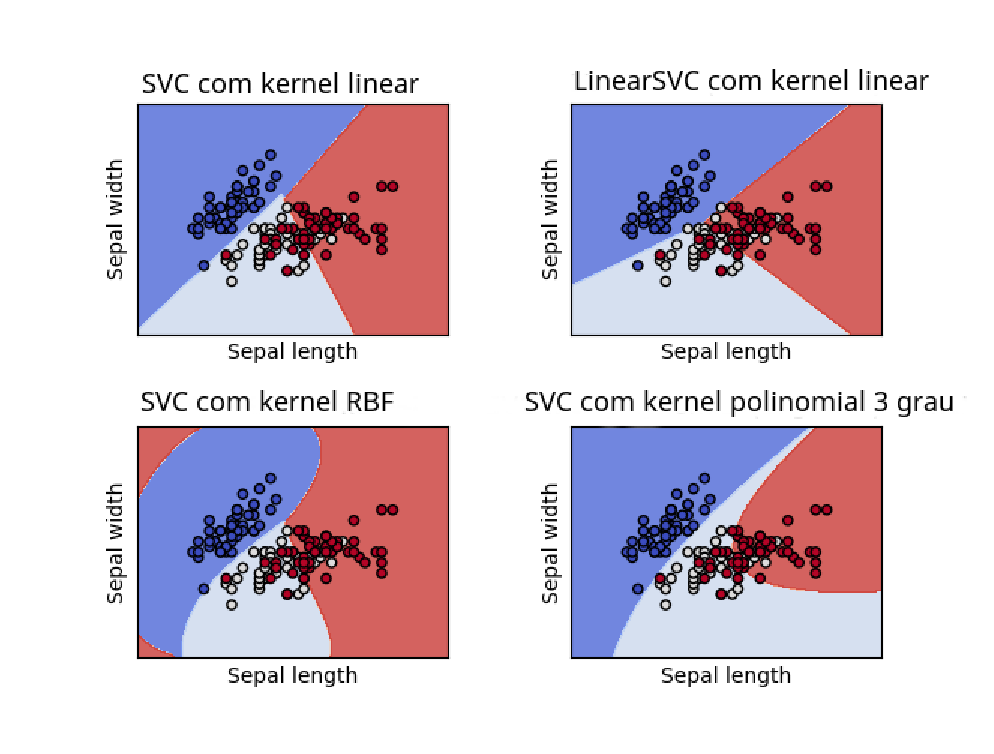
\includegraphics[width=0.9\textwidth]{figuras/svmkernel.eps}
     \caption{SVMs utilizando \textit{kernel} diferentes, adaptado de \citeonline{scikit-learn}}
     \label{svmkernel}
 \end{figure}

 \subsection{Funcionamento}

Um estudo \cite{wang2005support} sobre as teorias e aplicações do modelo, realizado por Theodoros Evgeniou e Massimiliano Pontil explicam bem a formulação do algoritmo se baseando nos estudos realizados por Vapnik para a construção modelo SVM. Este estudo será o guia para a explicação do funcionamento desse modelo nessa subseção.

Outro estudo realizado por Vayatis e Azencott \cite{vayatis99estimate} discute o arcabouço teórico básico no qual máquinas de aprendizagem como SVM foram desenvolvidas, e sugerem possíveis direções de pesquisa que podem levar a melhorias da teoria e possivelmente a melhorias de SVM como por exemplo a teoria pode ser usada para escolher os parâmetros de um SVM, como o seu kernel \cite{vapnik1998statistical}.
 
As SVMs foram desenvolvidas no âmbito da Teoria Estatística da Aprendizagem, logo para entender o funcionamento do dado modelo é necessário entender o próprio framework da Teoria Estatística da Aprendizagem \cite{vapnik1998statistical}, porém como o foco é esboçar o funcionamento do modelo, não será abordado de maneira aprofundada o conceito da Teoria Estatística da Aprendizagem neste trabalho cujo o foco é a implementação. 
 
Uma explicação simplista do funcionamento do SVM é a linear, na qual o hiperplano se encontra no espaço dos dados de entrada x. A noção mais comum sobre o SVM, é que o mesmo encontra um melhor hiperplano como a solução para o problema de aprendizagem \cite{vapnik1998statistical}. No caso linear o espaço de hipóteses é um subconjunto de todos os hiperplanos da forma \cite{wang2005support}:\[f(x)= w\cdot x +b\]
Em sua formulação mais geral, o SVM encontra um hiperplano em um espaço diferente daquele dos dados de entrada x. É um hiperplano em um espaço de característica induzido por um kernel K. Através do kernel K, o espaço de hipóteses é definido como um conjunto de "hiperplanos" no espaço de feições induzido por K. Isso também pode ser visto como um conjunto de funções em um Espaço Hilbert de Reprodução (RKHS) definido por K \cite{wahba1990spline}, \cite{vapnik1998statistical}. Também não será discutido aqui a RKHS neste trabalho, assim como o mesmo não é discutido no estudo \cite{wang2005support}. Então, para resumir, o espaço de hipóteses usado pelo SVM é um subconjunto do conjunto de hiperplanos definido em algum espaço de um RKHS. Este espaço pode ser formalmente escrito como.\[\left \{ f:\left \| f \right \|_{2}^{k} < \infty \right \}\]
Onde K é o kernel que define o RKHS, e $ \left \| f \right \|_{2}^{k} $  é a norma RKHS da função [21]. SVM considera os conjuntos da forma. \[\left \{ f:\left \| f \right \|_{2}^{k} \leq A^{2} \right \}\] para alguma constante A. Na estrutura da Teoria Estatística de Aprendizagem, a constante A é usada para definir uma estrutura de espaços de hipóteses (o quanto maior for, mais complexo é o espaço da hipótese). O objetivo do SVM é encontrar a solução com a norma RKHS "ideal", ou seja, encontrar o A ótimo \cite{wang2005support}.

A segunda opção retratada pelo estudo \cite{wang2005support} é a da função de perda, é uma função que mapeia um evento ou valores de uma ou mais variáveis num número real intuitivamente representando algum "custo" associado ao evento \cite{wald1950statistical}. O estudo \cite{wang2005support} distingue os classificadores SVM e regressores SVM, porém como este trabalho será focado na classificação, será apenas retratado o primeiro caso dos classificadores SVM.

Para classificação idealmente o erro de erro de classificação precisa ser minimizado, então uma função de perda do sinal de forma $ (-yf(x)) $ deve ser usada (na classificação y toma valores binários $ \pm1 $, e a classificação é feita tomando o sinal de função $ f(x) $). No entanto, devido à escala e às razões computacionais \cite{vapnik1998statistical}, a função de perda real usada para classificação SVM é $ |1-yf(x)|_{+} $ (ou seja, 0 se $ |1-yf(x)|< 0 $ e $ |1-yf(x)| $ caso contrário). Isso também é chamado de função de perda de "margem flexível" por causa de sua interpretação padrão de "margem": os pontos para os quais a função de perda é zero são os que têm "margem" \cite{wang2005support}.\[yf(x)/\left \| f \right \|_{k}^{2}\]

Para o caso $ 1/\left \| f \right \|_{k}^{2} $, ou seja, $1-yf(x) \geq  0 \Rightarrow yf(x)/\left \| f \right \|_{k}^{2} \geq 1/\left \| f \right \|_{k}^{2} $. A margem é uma quantidade geométrica importante associada à classificação SVM \cite{wang2005support}

SVM para classificação:
\[min\left \| f \right \|_{k}^{2}+C\sum_{i=0}^{l}\left | 1-y_{i}f(x_{i})\right |_{+}\]
